% Report for spring 2017 project for fys2130 waves and oscillations
\documentclass[12pt]{article}
\usepackage{amsmath}
\usepackage{graphicx}
\usepackage{float}
\usepackage[normalem]{ulem}
\usepackage{listings}

\title{spring 2017 Fys2130: waves and oscillations}
\date{}
\author{Candidacy number: 15040}

\begin{document}

%%%%%%%%%%%%	this would be where the header or front page goes	%%%%%%%%%%%%%%%
\maketitle

\includegraphics[scale=0.6]{UiOLogo}
\newpage
%%%%%%%%%%%	thus begins the actual project report
\section*{Project spring 2017, waves and oscillations}

We will investigate in greater detail waves along a string In order to accomplish this, we simulate the string with N discrete point-masses of mass \textit{m} connected with N-1 springs, each of which has a spring constant of \textit{k}.
\begin{figure}[hb]
	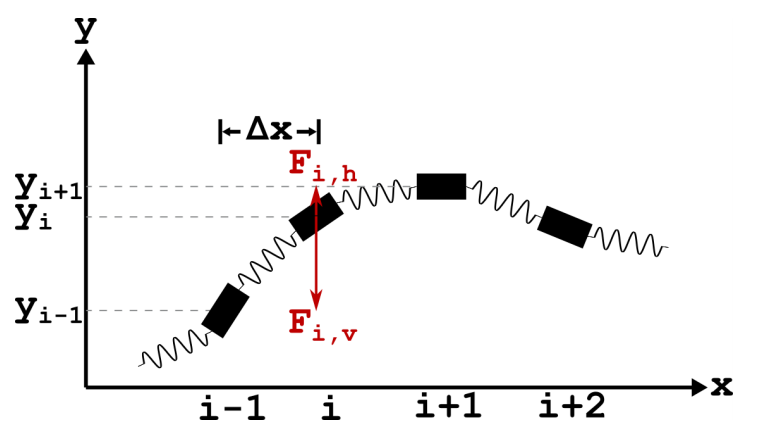
\includegraphics[scale=0.7]{DiscreteString.png}
	\caption{Discrete simulation of string. The point masses labeled from i=0, N-1
			pictured. There is no movement along the 1. axis. We do measure height in y-direction as
			seen with $y_{i-1},\; y_i,\; y_{i+1}$. As we do not measure any change in x-direction, our 
			only forces pull along the y-axis. Image taken from main project text. I will rename 
			$F_{i,h}$ and $F_{i, v}$ to $F_{i\pm1}$}
\end{figure}
Before jumping into the main work, I wish to define some equations we will be using:
$$ F_{i-1} = -k_{i-1}dy_{i,v} = -k_{i-1}(y_i - y_{i-1} $$
$$ F_{i+1} = -k_i dy_{i+1} = -k_i(y_i - y_{i+1})$$
\begin{equation}
\begin{aligned}
F_i = F_{i-1} + F_{i+1} = -(k_{i-1} + k_i)y_i + k_{i-1}y_{i-1} + k_iy_{i+1}
\end{aligned}
\end{equation}

We also have
\begin{equation}
\begin{aligned}
\ddot{y} = \frac{d^2y_i}{dt^2} \approx \frac{y_i^+ - 2y_i^0 + y_i^-}{(\Delta t)^2}
\end{aligned}
\end{equation}
where $y_i^-,\; y_i^0,\; y_i^+$ is previous, current and next timestep respectively

And finally, we have the motion equation 
\begin{equation}
	\begin{aligned}
		F_i = m_i\ddot{y_i}
	\end{aligned}
\end{equation}

\section*{Problem 1}
	To evolve the string's motion, we need to solve eq. (3) for $y^+$. We already know the details from 
eq.'s (1) and (2). Inserting these into (3) gives us:
\begin{equation}
	\begin{aligned}
		-(k_{i-1} + k_i)y_i + k_{i-1}y_{i-1} + k_iy_{i+1} &=
		 m_i \frac{y_i^+ - 2y_i^0 + y_i^-}{(\Delta t)^2} \\
		\text{Solving this with regards to $y_i^+$} \\
		\frac{\Delta t^2}{m_i}[ -(k_{i-1} + k_i)y_i^0 + k_{i-1}y_{i-1}^0 + k_iy_{i+1}^0 ] &= 
		y_i^+ - 2y_i^0 + y_i^- \\ \\
		y_i^+ = \frac{\Delta t^2}{m_i}[ -(k_{i-1} + k_i)y_i^0 + k_{i-1}y_{i-1}^0& + k_iy_{i+1} ]
				+ 2y_i^0 - y_i^-
	\end{aligned}
\end{equation}
There isn't a whole lot we can cut away here. We see the position at the next time-step will be dependent on the positions of the masses in the immediate vicinity as well as it's previous position. 
The ends of our string is a special case, as there will be only 1 spring acting on them. Thus we can simplify the expressions for this. 
\begin{equation}
	\begin{aligned}
		y_0^+ &= \frac{\Delta t^2}{m_0} [ -k_0y_0^0 + k_0y_1^0 ] + 2y_0^0 - y_0^- \\
		y_{N-1}^+ &= \frac{\Delta t^2}{m_{N-1}} [ -k_{N-2}y_{N-1}^0 + k_{N-2}y_{N-2}^0 ] 
					+ 2y_{N-1}^0 - y_{N-1}^-
	\end{aligned}
\end{equation}
Where the next and previous positions are removed accordingly. \\
	With the ends of our string open, we can utilize the equations as they are. Because the ends will swing and misalign any constant periods, there will be no constant nodes and wavelengths. Our system cannot disperse energy, however, and the oscillations will not die. \\
	In the event that we tie the ends of the rope to a wall or similar fixture, we then have total reflection, as we once again do not let the energy escape. The wave will invert it's amplitude, but otherwise traverse along the string in the opposite direction. This is effectively done by setting the masses at the end to be far greater than the remaining. $m_0 = m_{N-1} \gg m_i \,,\; i \in [1, N-2]$

\newpage
\section*{Problem 2}
	If we are to emulate the motions of a wave along a string, we need the wave equation. Since we are essentially modelling a string, we would normally use mass density and tension to model the velocity. If we incorporate this into our equations, we get $\mu = \frac{m_i}{\Delta x}$ and $\kappa = k\Delta x$ where $\Delta x$ is the distance between 2 point masses. Setting these into our equation (4) gives us
\begin{equation}
	\begin{aligned}
		-(k_{i-1} + k_i)y_i + k_{i-1}y_{i-1} + k_iy_{i+1} &=
				 m_i \frac{y_i^+ - 2y_i^0 + y_i^-}{(\Delta t)^2} \\
		\text{ With the definition of a constant tension }\\
		\text{along the string, we can simplify the 
			expression} \\
		k ( -2y_i + y_{i-1} + y_{i+1} ) &= m_i \frac{y_i^+ - 2y_i^0 + y_i^-}{(\Delta t)^2} \\
		\frac{\kappa}{\Delta x} ( -2y_i + y_{i-1} + y_{i+1} ) &= \mu \Delta x \frac{y_i^+ - 2y_i^0 + 
		y_i^-}{(\Delta t)^2} \\
		\text{From eq. (2), we know that the right side can be} \\
		\text{rewritten. A similar sollution exists for the left side} \\		
		\frac{\kappa}{\Delta x}(y_{i+1}^0 - 2y_i^0 + y_{i-1}^0) &= \mu \Delta x \frac{d^2y}{dt^2} \\
		\text{moving $\mu$ over to $\kappa$, we get this expression:} \\
		\frac{\kappa}{\mu \Delta x^2}(y_{i+1}^0 - 2y_i^0 + y_{i-1}^0) &= \frac{d^2y}{dt^2} \\
		\frac{d^2y}{dt^2} &= \frac{\kappa}{\mu} \frac{y_{i+1}^0 - 2y_i^0 + y_{i-1}^0}{\Delta x^2} \\
		\text{As we saw in eq. (2), this can be approximated to} \\
		\frac{d^2y}{dt^2} &= \frac{\kappa}{\mu}\frac{d^2y}{dx^2} \\
		\text{This is the wave equation, and it thus follows, that} \\
		\frac{\kappa}{\mu} &= v_B^2 \\
		\frac{d^2y}{dt^2} &= v_B^2\frac{d^2y}{dx^2} \\
	\end{aligned}
\end{equation}
With this, we can see that our motion equation follows the wave equation, and our model should behave like a wave.
\section*{Problem 3}
In order for us to model this string the script needs to have a high enough resolution. This means that the numerical $\frac{\Delta x}{\Delta t}$ has to be greater than $v_B$. thus:
\begin{equation}
	\begin{aligned}
		\frac{\Delta x}{\Delta t} &> v_B \\
		\frac{\Delta x}{\Delta t} &> \sqrt{\frac{k}{m}} \Delta x \;\;|\;\;
		\text{We can remove the $\Delta x$} \\
		\frac{1}{\Delta} &> \sqrt{\frac{k}{m}} \;\;|\;\; \text{We know $\Delta t > 0$} \\
		\Delta t &< \sqrt{\frac{m}{k}}
	\end{aligned}
\end{equation}
	Thus, we need to make sure our numerical time-step is less than $\sqrt{\frac{m}{k}}$ in order to ensure that we can accurately model the waves. A simple way to do this, is to use 
$\Delta t = \epsilon\sqrt{\frac{m}{k}}$ for $\epsilon < 1$. \\
	with an initial $\epsilon=0.8$. This $\epsilon$ is mostly arbitrary, as long as it does not exceed 1. While working, I found that a higher epsilon lent itself better to my solutions. In the extreme, I sett $\epsilon = 1$ on the final problem. Aside from the strictly practical interface with my particular solution, the resolution of the program needs to ensure the capture of all motion. This large $\epsilon$ has not noticeably deteriorated the accuracy of the estimations

\section*{Problem 4}
	We should have what we need to begin our model now. We define a string of $N = 200$ point masses, each with a mass $m = 0.02kg$ and $N-1$ springs with spring constants $k_i = 10\frac{kg}{s^2}$. We define a timestep distance $dt = \epsilon\sqrt{\frac{m}{k}}s$. \\
	Initially, we will evaluate a standing wave of shape
\begin{equation}
	\begin{aligned}
		y_i^0 = sin(7\pi\frac{i}{N-1}) \;, \;\; i\in [0, N-1]
	\end{aligned}
\end{equation}
In addition, to ensure a standing wave, we also need to fasten the ends. Therefore, we set $m_0 = m_{N-1} \gg m$. Initially, we run the simulation over 1200 timseteps. \\
	We also initialize the timestates of y as a 2D array of Nxt elements. As such, we rewrite the functions (4) and (5) from problem 1.
\begin{equation}
	\begin{aligned}
		y_{i, t+1} &= \frac{\Delta t^2}{m_i}[ -(k_{i-1} + k_i)y_{i, t} + k_{i-1}y_{i-1, t} + k_iy_{i+1, t} ]
				+ 2y_{i, t} - y_{i, t-1} \\
		y_{0, t+1} &= \frac{\Delta t^2}{m_0} [ -k_0y_{0, t} + k_0y_{1, t} ] + 2y_{0, t} - y_{0, t-1} \\
		y_{N-1, t+1} &= \frac{\Delta t^2}{m_{N-1}} [ -k_{N-2}y_{N-1, t} + k_{N-2}y_{N-2, t} ] 
					+ 2y_{N-1, t} - y_{N-1, t-1}
	\end{aligned}
\end{equation}

	Seeing as (8) is a sine function, wich can be said to have a \\$(kx + \omega t) = 7\pi\frac{i}{N-1}$ and we should expect to see, as mentioned above, a harmonious wave.\\
	if we also go by $\lambda = 2\pi x$, we should expect roughly 3.5 periods. The nodes here, should be constant, as we neither lose energy, nor transmit any waves. Due to the function being a trigonometric one, The amplitudes should move from -1 to 1.
	Using these assumptions, we can state that the previous timestate should be within the standing wave's configuration. The nodes will be constant. We also know, that this initial state will be an extremal point. In that case, the starting velocity will be zero. Thus, the previous time step should be equal to the present. This could also be thought off as us starting the system out this way, simply by "pulling" the string into this position and watching the movement unfold. \\
	The script initializes firstly all the relevant variables to the system. I store mass, spring constants and positions in arrays of Nx1 and Nxnt for the values and positions respectively.
	%sett inn og forklar endringen i algoritme fra opg. 1
	 The first act is to set the 2 first rows of my position array to be our sin function. When developing the system in time, I apply the motion equation with special regards to the end points from problem 1. Next, I loop over the remaining points on the string with the general motion equation from (9). Having gone through all time-steps, I animate the movement to visualize the motion, before storing 3 plots of various states along the timespan of the motion. \\
	Running the script also produces much of the expected evolution, with the initial excitation of the sin function, which then oscillates between the constant nodes, alternating tops and valleys. Figures 2 and 3 displays the extreme points of this, where in between the differences are the amplitudes. 
	
\begin{figure}[ht]
	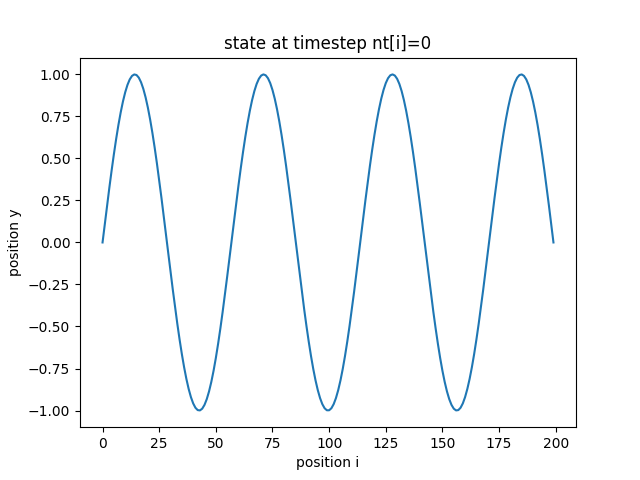
\includegraphics[scale=0.7]{state_timestep_0}
	\caption{This is a snapshot of the oscillations along the string following the sin function. The snapshot is taken at time t=0. We can see approximately 3.5 wavelengths along the string, and a maximal excitation of 1. The 1. axis depicts the position along the string as point mass 1, 2,... and so on, not any specific unit of space.}
\end{figure}
%%% insert figure for t=15, where the amplitude is almost 0?
\begin{figure}[H]
	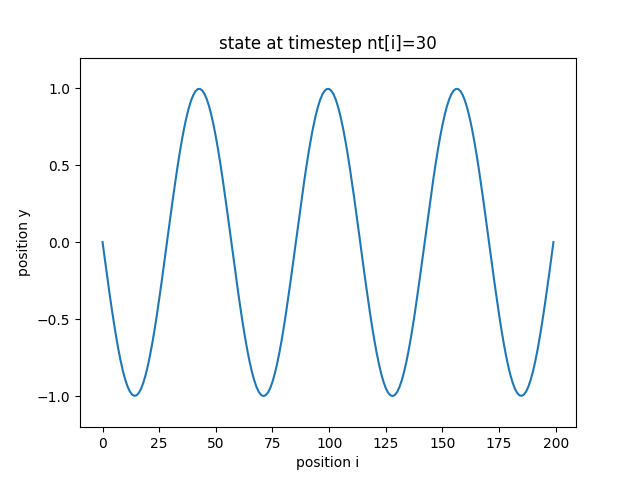
\includegraphics[scale=0.7]{state_timestep_30}
	\caption{This is a snapshot of the same string 30 timesteps later. We can notice that the amplitudes have been reversed, as this is the second extreme state between which the system oscillates.}
\end{figure}


\section*{Problem 5}
	The oscillations of the string should hold a predictable frequency. We know that the frequency can be written as $\frac{v}{\lambda}$. we already know the velocity, $v_B = \sqrt{\frac{k}{m}} \Delta x$, and we next need to find the wavelength. We predicted and also noticed on the plot, that the string had roughly 3.5 wavelengths along it's length. Thus we can find $\lambda = \frac{x}{3.5}$ where $ x = N \cdot \Delta x$. We can then find $f = \sqrt{\frac{k}{m}}\frac{\xout{\Delta x}}{\xout{\Delta x} \cdot 200}\cdot 3.5$ which gives us a frequency of $f = 0.39s^{-1}$. \\
	To view our oscillations in a different dimension, we wish to show the excitation of the 100th element of the string over 10 periods. As such, we need to know both how much time 10 periods span, and how many timesteps this corresponds to. A simple fix for this, is to find the total time for 10 periods $T_{10} = \frac{10}{f}$ and then extracting the number of timesteps from this with $n_{10} = int(\frac{T_{10}}{\Delta t})+1$. \\
	I scripted this and picked out the $n_{10}$ first elements of the 100th collumn of my y. While I initially opened a .npy file I had stored all timestates in, I have recreated the motions in this script. This is for the readability and simplicity of testing. This does reduce the effectiveness of the script a little. I believe the reduction is negligible due to the comparatively small number of data-points compared to current computational speed. \\
	After recreating the positional array, I choose the $n_{10}$ first elements of the 100th collumn and plot them, see figure 4. zooming in and reading off a small interval around the first 2 maxima, I then find the exact maximal values, and store them and their index. Using the difference between the 2 maxima, I multiply it with the step length of each timestep to find the discrete period. I next find the proportional error between the expected frequency and the discrete frequency. The error comes out to $0.5\%$ which is within acceptable range. \\
	Next, I perform a frequency analysis using the fast fourier transform method. Scanning the resulting array for the index of it's maximal value, I compare it with a frequency array I set up and check the proportional difference to my expected frequency. There is an error of $0.2\%$ which once more lies well within acceptable levels of divergence. Finally, I plot the fft.
	
\begin{figure}
	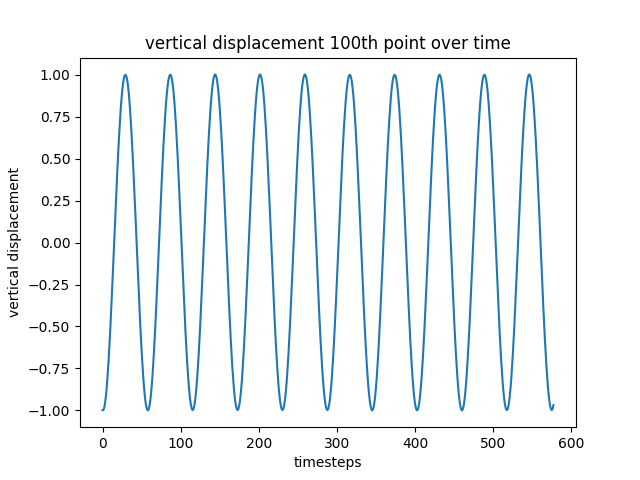
\includegraphics[scale=0.7]{y99_OverTime}
	\caption{We see the oscillations follows roughly the same shape as the spatial propagation of the wave. This is another indication that the motion follows the wave equation. We can also read out a rough period of 50 timesteps. }
\end{figure}

\begin{figure}
	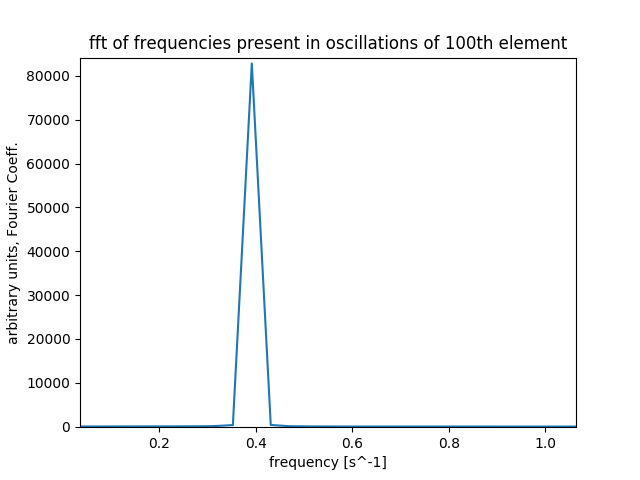
\includegraphics[scale=0.7]{fft_y99_OverTime}
	\caption{A zoomed in image of the fft of the system. We see that the spike appears close to, but perhaps just shy of $0.4s^-1$. The values along the y-axis should be regarded as largely arbitrary due to squaring the conjugate norm of a complex array.}
\end{figure}

\section*{Problem 6}
	We have observed that the simulation has a seemingly constant amplitude and wavelength. In order to completely establish this, we need to make sure the energy is conserved. We know that $E = K + V$, and that $K = \frac{1}{2}mv^2$ and, for a spring, $V = \frac{1}{2}k\Delta x^2$. In order to ensure that energy is maintained across the string for all times in which we simulate, we need to make an algorithm for these energies. \\
	Beginning with kinetic, we notice that most of it is simple enough to implement, but we need an approximation to the velocity. In order to center the approximation on the current time, I use the previous and the next timestep and divide the distance over the double timestep. the final algorithm then becomes 
	
\begin{equation}
	\begin{aligned}
		K_i = 0.5m_i(\frac{y_{i, t+1} - y_{i, t-1}}{2dt})^2 \\
		V_i = 0.5k_i(y_{i+1, t} - y_{i, t})^2
	\end{aligned}
\end{equation}
	
	We want the kinetic energy of all point masses, and we iterate this over all timestates, except the first and final. This is due to the final step lacking required information. We also need the energy stored in each spring and we iterate over the $N-1$ springs. \\
	The initial timestep is as we are starting. Because this is an exremal point, we know that this instant, there is no kinetic energy, Therefore the first stage is pure potential. As we evolve the state through time, we check the final energy and the error in the difference with the initial. \\
	the results come out to an initial energy of $E_0 = 6.069$ and a final energy of $E_{end} = 6.075$ which results in an error of $error = 0.1\%$. This seems to be a pretty good fit, and as we can see on figure 6, the energy lies rather stably. 
	
\begin{figure}[H]
	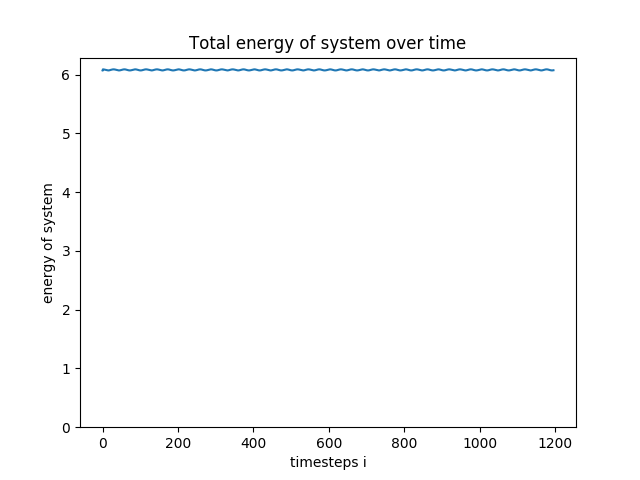
\includegraphics[scale=0.7]{SystemEnergy}
	\caption{We see that the total energy of the system in our model weaves up and down slightly around 6. Some wobble is to be expected when dealing with discrete positions. It is truncated from the 1st and last points on the string, because the end-points were causing trouble}
\end{figure}

\section*{Problem 7}
	To explore our simulation further, let us study a progressing pulse with a triangle shape. Initially, we generate the triangle in the middle of the string and evolve the state over time. We maintain the reflecting endpoints. \\
	As we evolve, we notice that the triangle's apex collapses down into 2 child waves, each of half the amplitude of the mother wave. This is not surprising, considering that the top pointmass has forces solely pointing downwards. \\
	The child waves seem to be an application of the superposition principle, combining to form 1 large wave at 1 point, and then split once more.  

\begin{figure}[H]
	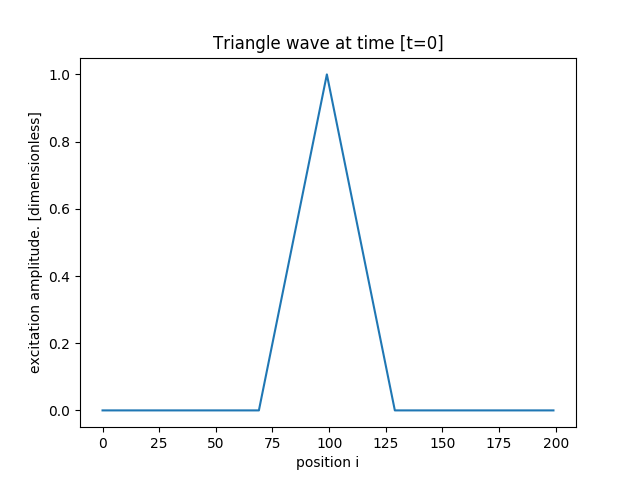
\includegraphics[scale=0.7]{TriangleWave_t0}
	\caption{Triangle wave at it's inception. Currently no time has passed, and the propagations are about to begin.}
\end{figure}

\begin{figure}[H]
	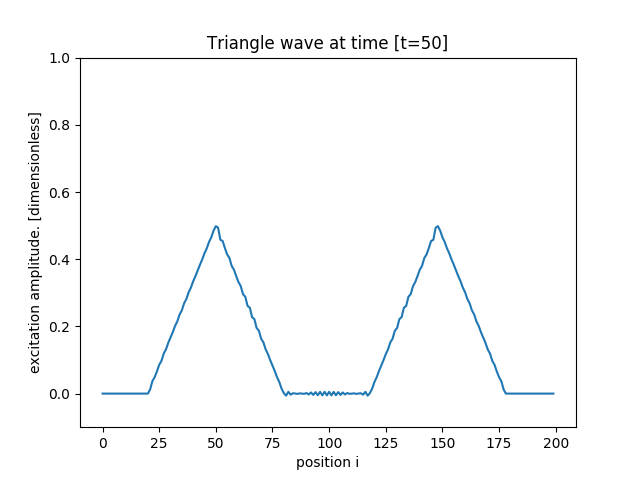
\includegraphics[scale=0.7]{TriangleWave_t50}
	\caption{Here we see the the initial pulse has split into to waves, each at half the original amplitude. The waves each have a velocity away from eachother. They will meet again once they have been reflected.}
\end{figure}

\section*{Problem 8}
	Now, we want to make the situation a little more exclusive. Therefore, we center the triangle wave to have it's maximum at i=3o, which means that the tail end ends just at the i=0. We also initialize the pulse with a velocity towards the right, which ensures it does not collapse. My solution is to manually move the wave 1 pointmass along. \\
	To ensure that the program proceeds smoothly after this, I approximate the timestep to be very close to the wave's velocity. This retains a high enough resolution, yet allows artefacts from the manual move to decrease sharply. 

\begin{figure}[H]
	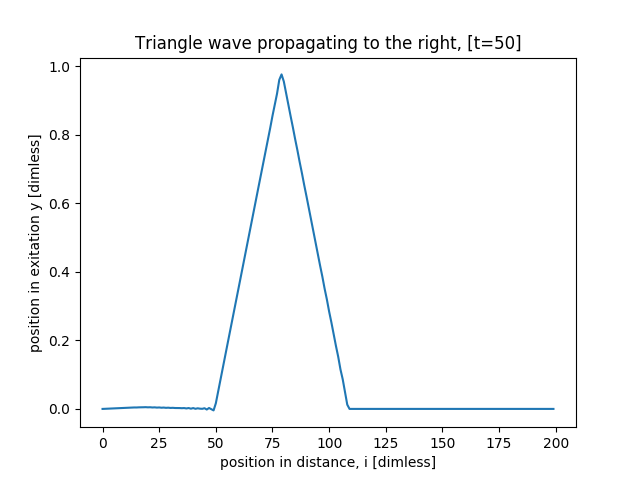
\includegraphics[scale=0.7]{TriangleWave_velocityRight}
	\caption{We see the wave som ways off from the inintial position. There are some rather minor artefacts tailing the wave. This results from timestep length that is less than the propagation velocity of the wave. Thus the initial condition is a little further ahead of the natural derivatives. }
\end{figure}	
	
\section*{Problem 9}
	As a final test, we elongate the rope, but the new part is a lot thicker. Thus, we have a thin thread tied to a larger one. We double the total number of point masses, and triple the mass per point in the new rope.\\
	The different masses of the 2 strings will result in an impedance for the power going through the compound string. This will result in partial transmition and reflection. The proportional difference between the impedances of the 2 strings will define how much energy is in each of the resulting waves.\\
	In order to measure this, I used the formulas and ideas about light reflecting and transmitting off of surfaces. This formula is $\frac{E_r}{E_i} = \frac{(n_1 - n_2)}{(n_1 + n_2)}$, which we can remodel to $\frac{n_1}{n_2} = \frac{E_t}{E_i - E_r}$, where the E's represent the amplitude of the reflected light, and the n is the relationship between the light speed in a vacuum and in the current medium. In other words, it is highly dependent on the velocity of the waves entering. \\
	For our string, the velocity difference is decided by the different masses, and so our impedance difference relation then becomes 
	\begin{equation}
		\begin{aligned}
			\frac{Z_1}{Z_2} = \frac{A_t}{A_i - A_r}
		\end{aligned}
	\end{equation} 
	Another way to verify this, is to look at the fact that both light and the waves along our string follow the same wave equation. 
	The script is modified with new initial values, where the length now is set to 400, and the masses above nr. 200 is trippled. In addition, I run the triangle wave along the compound rope. After evolving the wave over time, I animate the motion. Then I choose snapshots, 1 before the reflection and 1 afterwards. I run a test to find the maxima and minima for the incident, reflected and transmitted wave. After this, I use the resulting amplitudes to find the relationship between the impedance as in (9). From chapter 7, we have accoustic impedance defined as $Z0 = \rho c$ with $\rho$ being the mass density and c the speed of sound. Once more, this is analogous to our representation on the string. We also know that the sound waves also follow the wave equation. Thus, we can substitute $\mu = \frac{m}{\Delta x}$ as mass density and $v_B$ as the velocity. This also has the handy feature of removing the $\Delta x$, finalizing the equation as
\begin{equation}
	\begin{aligned}
		Z_i = \sqrt{m_ik_i}
	\end{aligned}
\end{equation}
With this, we can get a sense of the error in the models propagation compared to the theoretical value. This is a good check, as it turns out, that the modelled impedance relation is at $0.555$, while the analytic method suggested $0.557$. This results in an error of $3.8\%$. I have modelled this string with a timestep resolution of just the same as $v_B$, and I have noticed that the error rises sharply once I reduce the step-length. This likely means that my initial propagation of the wave, through manually adjusting it a step ahead in time has some incongruencies. These are compounded if the difference between the waves propagation over time between the first 2 steps and the further natural steps. 

\newpage
\section*{appendix}
\newpage
	\subsection*{problem 4}
		\lstinputlisting{opg_4.py}
\newpage
	\subsection*{problem 5}
		\lstinputlisting{opg_5.py}
\newpage
	\subsection*{problem 6}
		\lstinputlisting{opg_6.py}
\newpage
	\subsection*{problem 7}
		\lstinputlisting{opg_7.py}
\newpage
	\subsection*{problem 8}
		\lstinputlisting{opg_8.py}
\newpage
	\subsection*{problem 9}
		\lstinputlisting{opg_9.py}
\end{document}